\section{Proofs and numerical checks}
\label{app:proofs}
\appendixnumbering

\paragraph{Notation and assumptions} For a gap $\Iset=(e_A,s_B)$ of length $\tau$ before event B with duration
$D_B$, let $\eta=\eta_{\mathrm c}\eta_{\mathrm d}$ be the round-trip efficiency (for the TES $\eta^{\mathrm{TC}}\eta^{\mathrm{TD}}$).
Propositions~\ref{prop:bound} and Theorem~\ref{thm:closed} use two assumptions. (H1) Unbiased baseline: without
response the import equals the baseline and the storage is idle in the gap and in event B. (H2) $\varepsilon_t$ and
$\COP_t$ are constant on $\Iset\cup\Tset_B$; otherwise all bounds hold with the largest $\varepsilon$ on that interval
and become slightly looser. Proposition~\ref{prop:region} does not need H1. Under H1, \eqref{eq:cool}--\eqref{eq:elec}
give the deviation of any schedule from the baseline as
\begin{equation}
\Pg_t-\Pb_t=\varepsilon\sum_c\Big(y_{c,t}-\frac{a_{c,t}}{\dt}\Big)+\Pch_t-\Pdis_t+\frac{\Qtc_t-\Qtd_t}{\COP}-\Delta g_t ,
\label{eq:deviation}
\end{equation}
where $\Delta g_t\in[0,g]$ is the additional gas-engine output including its absorption cooling.

\paragraph{Proof of Lemma~\ref{lem:edf}} For one class, let $x_t=y_t\dt$, $A_t=\sum_{s\le t}a_s$, $X_t=\sum_{s\le
t}x_s$, $B_t=A_t-X_t\ge0$, and let $D_t=\sum_{\tau\le t-L/\dt}a_\tau$ be the work due by step $t$, so that
$\Bbar_t=A_t-D_t$. (i)$\Rightarrow$(iii): all work due by $t$ (amount $D_t$) has been executed by $t$, hence $X_t\ge D_t$,
\ie\ $B_t\le\Bbar_t$. (iii)$\Rightarrow$(ii): EDF serves the batches in the order of arrival, so the first $D_t$ units of
execution fall on the batches due by $t$, and $X_t\ge D_t$ completes them in time; since $B_t\ge0$, EDF never executes
work that has not arrived. (ii)$\Rightarrow$(i) is immediate. With several classes sharing the GPUs the argument holds
class by class, because the capacity \eqref{eq:gpucap} only limits $\sum_cy_{c,t}$. A constant limit $\bar Q$ admits
overdue work whenever $\bar Q>\Bbar_t$ and excludes feasible deferrals whenever $\bar Q<\Bbar_t$. $\square$

\paragraph{Proof of Proposition~\ref{prop:bound}} (i) Restricting any feasible schedule of the two-event problem to event
B gives a feasible schedule of the problem with event B alone and the same initial state, hence $\Gamma_B\le\Gamma_B^0$.
(ii) Summing \eqref{eq:deviation} over $\Tset_B$ and using the backlog equation \eqref{eq:backlog},
\begin{multline*}
\Gamma_BD_B=\varepsilon\sum_c\big[B_c(e_B)-B_c(s_B^-)\big]\\
+\sum_{t\in\Tset_{B}}\Big(\Pdis_t-\Pch_t+\frac{\Qtd_t-\Qtc_t}{\COP}\Big)\dt+\sum_{t\in\Tset_{B}}\Delta g_t\dt .
\end{multline*}
By \eqref{eq:lag} the first term is at most $\bar X_B-X(s_B^-)$, the second at most the dischargeable energy $E_s(s_B^-)$,
and the third at most $gD_B$. In the gap, let $C_{\Iset}=\varepsilon\sum_{t\in\Iset}\sum_c(y_{c,t}\dt-a_{c,t})$ be the net
catch-up and $D_{\Iset}$ the net storage intake. Summing \eqref{eq:deviation} over $\Iset$ with $\Pg_t\le\Pcap$ gives the
channel constraint $C_{\Iset}+D_{\Iset}\le H$. Moreover $X(s_B^-)=X_A-C_{\Iset}\ge0$ and $E_s(s_B^-)\le E_s+\phi(D_{\Iset})$ with
$\phi(x)=\eta x$ for $x\ge0$ and $\phi(x)=x$ for $x<0$. Hence
$\Gamma_BD_B-gD_B\le\bar X_B-X_A+E_s+\max\{C+\phi(D):C+D\le H,\ C\le X_A\}$. Catch-up has marginal value one and
recharging $\eta<1$ (discharging in the gap has value one but costs the same amount of catch-up), so the maximum is
attained by catching up first, $C^*=\min(H,X_A)$, and recharging with the rest, which gives $H_{\mathrm{eff}}$ and
\eqref{eq:bound}. (iii) In event B the computing reduction equals the backlog increase. New arrivals of class $c$ can be
deferred by at most $\min(L_c,D_B)$, which bounds this increase by $p_fD_B$ with
$p_f=\varepsilon\sum_c\bar a_{c,B}\min(L_c,D_B)/D_B$. The backlog $X_A^{\mathrm{due}}$ that falls due before $e_B$ must be
caught up in the gap ($H_c$), or exchanged by EDF with new work whose deadline lies after $e_B$ (at most $W_{\mathrm{sw}}$),
or executed in B, offsetting reduction. The storage reduction is limited by the power $P_s$ and the energy
$E_s+\eta H_s$. Allocating the channel $H_c+H_s\le H$ under the idle GPU capacity $G^{\mathrm{free}}$ and the charging
power gives the power-type bound
\begin{multline}
\Gamma^{\mathrm P}=g+\max_{\substack{H_c+H_s\le H\\ H_c\le\varepsilon G^{\mathrm{free}}\tau,\ H_s\le\bar P^{\mathrm B}\tau}}
\Big\{p_f-\frac{(X_A^{\mathrm{due}}-H_c-W_{\mathrm{sw}})^+}{D_B}\\
+\min\Big(P_s,\frac{E_s+\eta H_s}{D_B}\Big)\Big\}. \quad\square
\label{eq:boundP}
\end{multline}

The energy bound is tight when the backlog reaches its deadline capacity at the end of B, the storage is emptied in B
and the gap uses the whole channel for catch-up first. It extends to further recovery states. Data hall thermal
inertia enters like the TES: the heat stored at $e_A$ is a recovery need $X^\Theta_A=\Theta_A/\COP$, the remaining
warm-up allowance is reusable in B, and removing 1~MWh$_{\mathrm{th}}$ of stored heat in the gap restores one unit of
allowance at efficiency one, so catch-up, heat removal and recharging all draw on $H$, ranked by marginal values 1, 1 and
$\eta$. A hot-water tank limits the cost of heat supply rather than the capability, and its marginal value in the gap is
$\lambda_t/\COP^{\mathrm{HP}}$. For rigid jobs, the catch-up in the gap is further limited by
$\bar C=\varepsilon\sum_cB_c(e_A)(1-e^{-\tau/\tau_c})$, and the optimal allocation becomes $C^*=\min(H,X_A,\bar C)$ with
$H_{\mathrm{eff}}=C^*+\eta(H-C^*)$: more of the channel can only recharge storage, which penalises independent recovery
most.

\paragraph{Proof of Theorem~\ref{thm:closed} and Corollary~\ref{cor:novalue}} With catch-up $c\le X$ and recharge intake
$s$, $c+s\le H$, the deliverable reduction energy of B is $G(c,s)=\min(p_fD_B,\,p_fL-(X-c))+\min(P_sD_B,\,\eta_{\mathrm d}E_A+\eta s)$.
The first term is concave piecewise linear with slope one for $c<c^*$ and zero afterwards (B can then pause its whole
deferrable load), the second has slope $\eta$ for $s<s_{\mathrm{req}}$ and zero afterwards. Maximising the sum of two
separable concave functions under $c+s\le H$ allocates greedily by marginal value: first $c$ up to $c^*$, then $s$ up to
$s_{\mathrm{req}}$, which is the JR allocation of (i). IR raises $c$ to $X$ first, so the channel spent on $X-c^*$ has no
value. Substituting both allocations gives \eqref{eq:dG}: the two are equal for $H\le c^*$, JR gains
$\eta\min(s_{\mathrm{req}},H-c^*)$ for $H>c^*$, and the gap narrows once IR starts to recharge at $H>X$; the maximum
$\eta\min\{X-c^*,s_{\mathrm{req}}\}$ is attained for $H$ between $\min(X,c^*+s_{\mathrm{req}})$ and $\max(X,c^*+s_{\mathrm{req}})$,
and $X-c^*=\min\{X,p_f(L-D_B)\}$. The stand-alone capability $p_fD_B+P_sD_B$ is reached if and only if $c\ge c^*$ and
$s\ge s_{\mathrm{req}}$, so JR and IR need the channel energies $c^*+s_{\mathrm{req}}$ and $X+s_{\mathrm{req}}$; dividing
by $h$ gives \eqref{eq:tau}. Corollary~\ref{cor:novalue} lists exactly the cases in which the two allocations coincide.
Two further consequences follow. Since $\tau^*h$ is constant, iso-capability curves are hyperbolas in the $(\tau,h)$
plane, so a longer gap and a larger connection headroom substitute for each other, and JR saves the channel energy
$\min\{X,p_f(L-D_B)\}$. Allowing additional pauses in the gap to free the channel for the storage ($c<0$) enlarges only
the feasible set of JR, so the theorem gives a lower bound on its advantage. With several classes, JR catches up only
$\sum_c[X_c-p_{f,c}(L_c-D_B)]^+$ and carries the long-lag backlog. $\square$

\begin{figure*}[!t]
\centering
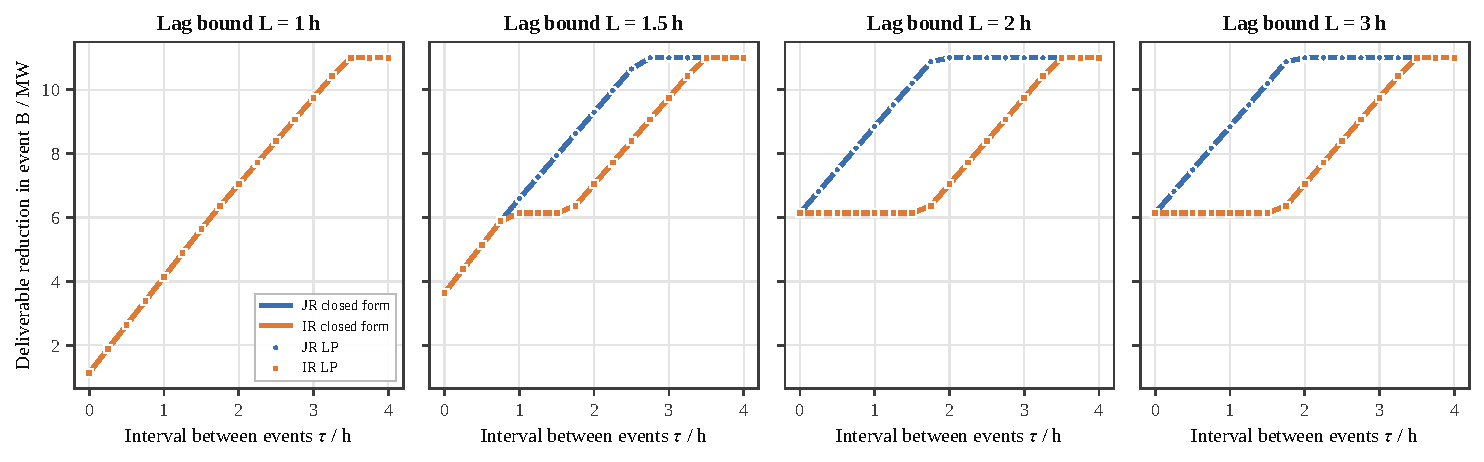
\includegraphics[width=\textwidth]{fig12_stylized_theorem.pdf}
\caption{Numerical check of Theorem~\ref{thm:closed}: closed form (lines) and discrete-time LP (markers) of the
deliverable reduction in event B ($p_f=5$~MW, $D_B=1$~h, $X=5$~MWh, $P_s=6$~MW, $E_A=1.2$~MWh,
$\eta_{\mathrm c}=\eta_{\mathrm d}=0.95$, $h=3$~MW; 68 cases, maximum deviation $10^{-5}$~MW).}
\label{fig:theorem}
\end{figure*}

\paragraph{Proof of Proposition~\ref{prop:price}} All statements are stationarity conditions of the LP with fixed
binaries. For $\Pch_t$, with cost $\cdeg\dt$, coefficient $-1$ in the electricity balance and $-\eta_{\mathrm c}\dt$ in
the energy equation $E_t-E_{t-1}-\eta_{\mathrm c}\dt\Pch_t+\dt\Pdis_t/\eta_{\mathrm d}=0$, a zero reduced cost at an
interior value gives $\cdeg\dt+\lambda_t\dt-\eta_{\mathrm c}\dt\nu_t=0$; discharging is analogous. The variable
$y_{c,t}$ has no own cost and appears in the backlog equation (coefficient $\dt$), the electricity balance
($-(1+a^{\mathrm{aux}})\pdyn$), the cooling balance ($-\theta\pdyn$) and the GPU capacity; with an interior electric
chiller the cooling dual equals $\lambda_t/\COP_t$, and with free GPU capacity its dual is zero, which gives
$\mu_{c,t}=\varepsilon_t\lambda_t$. Stationarity in $\Pg_t$ gives the decomposition of $\lambda_t$, and stationarity in
$B_{c,t}$ gives $\mu_{c,t}=\mu_{c,t+1}+\cjct\dt-\delta_{c,t}$, where the deadline dual $\delta_{c,t}\ge0$ is non-zero only
when the backlog reaches its bound. Combining the conditions yields \eqref{eq:equalmarginal}. $\square$

\paragraph{Proof of Proposition~\ref{prop:dro}} Fix $x$ and write $f_\omega=f_\omega(x)$. With $u_\omega\ge|p_\omega-\hat
p_\omega|$ the inner problem is the LP $\max\sum_\omega f_\omega p_\omega$ subject to $\sum_\omega p_\omega=1$ (dual
$\eta$), $p_\omega-u_\omega\le\hat p_\omega$ ($\alpha_\omega\ge0$), $-p_\omega-u_\omega\le-\hat p_\omega$ ($\beta_\omega\ge0$)
and $\sum_\omega u_\omega\le\delta$ ($\nu\ge0$). Its dual is $\min\eta+\sum_\omega\hat p_\omega(\alpha_\omega-\beta_\omega)+\delta\nu$
subject to $\eta+\alpha_\omega-\beta_\omega\ge f_\omega$ and $\nu\ge\alpha_\omega+\beta_\omega$. With
$\lambda_\omega=\alpha_\omega-\beta_\omega$, the minimum of $\alpha_\omega+\beta_\omega$ is $|\lambda_\omega|$, so the
constraints become $|\lambda_\omega|\le\nu$. The primal is feasible ($p=\hat p$) and bounded, so strong duality holds and
the inner maximum can be replaced by this minimum, which turns \eqref{eq:dro} into a single minimisation with
$f_\omega(x)\le\eta+\lambda_\omega$. Because $f_\omega(x)$ is itself a minimum over $y_\omega$ and the constraint is
monotone in $f_\omega$, ``there is $y_\omega\in\mathcal Y_\omega(x)$ with $c_\omega^\top y_\omega\le\eta+\lambda_\omega$''
is equivalent to $f_\omega(x)\le\eta+\lambda_\omega$, which gives \eqref{eq:droR}. For $\delta=0$, $\nu$ is free and
$\lambda_\omega=f_\omega-\eta$ yields $\sum_\omega\hat p_\omega f_\omega$ (SP); for $\delta\ge2(1-\min_\omega\hat p_\omega)$,
$\mathcal P_\delta$ contains every point mass and the inner maximum is $\max_\omega f_\omega$ (RO). Moving probability
from the cheapest scenarios to the most expensive one is the greedy solution of the inner LP, whose value is concave and
piecewise linear in $\delta$ with slopes $(f_{\bar\omega}-f_\omega)/2$; $V(\delta)$, the infimum of such functions over
$x$, is non-decreasing and concave, and with fixed binaries $\nu^*$ is a supergradient by the envelope theorem.
$\mathrm{CVaR}_\beta$ corresponds to $\{p:0\le p_\omega\le\hat p_\omega/(1-\beta),\sum_\omega p_\omega=1\}$ and is linearised
by $\mathrm{CVaR}_\beta=\min_\eta\eta+\frac1{1-\beta}\sum_\omega\hat p_\omega(f_\omega-\eta)^+$~\cite{rockafellar2000}. $\square$

\paragraph{Proof of Proposition~\ref{prop:region}} (i) Delivering $C$ means that $(C,x)$ satisfies linear constraints:
the joint model, no overdue work, $\Pg_t\le\Pcap$, mean reductions of at least $C_k$, and $C\ge0$. $\Cset$ is the
projection of this polyhedron on $C$ and therefore a convex polyhedron. It is downward closed because a reduction of at
least $C_k$ is also at least $C'_k\le C_k$, contains the origin when non-empty, and $C\in\Cset$ implies
$(0,\dots,C_k,\dots,0)\in\Cset$, hence $C_k\le\Gamma^0_k$, which gives $\Cset\subseteq\mathcal B$ and boundedness. (ii)
The second stage of a sequential strategy is the joint model with the IT plan fixed, so its feasible operations are
feasible for the joint model. (iii) Writing the import as
$\Pg_t=P^{\mathrm{nom}}_t+\varepsilon\sum_c(y_{c,t}-a_{c,t}/\dt)+\Pch_t-\Pdis_t+(\Qtc_t-\Qtd_t)/\COP-\Delta g_t$ (plus PV
curtailment, which only raises the import) and summing over the events of $S$,
$\sum_{k\in S}D_kC_k\le\Delta_S+\varepsilon[\text{backlog increase in the events}]+[\text{net storage discharge in the
events}]+gD_S$. The backlog increase equals $X(e_j)-X(s_i^-)+\sum_{\Iset} C_{\Iset}\le\bar X(e_j)+\sum_{\Iset} C_{\Iset}$ by
Lemma~\ref{lem:edf}; the net discharge is at most $E_s^{\max}+\sum_{\Iset} D_{\Iset}$ because $\phi(x)\le x$; and in every
gap $C_{\Iset}+D_{\Iset}\le\sum_{t\in\Iset}[(\Pcap-P^{\mathrm{nom}}_t)^++g]\dt$. Adding the three inequalities gives
\eqref{eq:multibound}. (iv) Every constraint of $\mathcal T$ is valid for $\Cset$, so $\Cset\subseteq\mathcal T$. For a
vertex $v$, $\theta^*\le\theta_v$, $\theta_vv\in\Cset$ and $0\in\Cset$, so convexity gives $\theta^*v\in\Cset$ and
$\theta^*\mathcal T=\mathrm{conv}\{\theta^*v\}\subseteq\Cset$. (v) The solver's response is one element of the optimal
response set, which gives the first inclusion; the second follows from (ii). Membership in $\Cset_{\mathrm{IR\text{-}P+}}$
is the feasibility of one LP that stacks the joint model for $C$ and the IT model for the price, equates their IT plans
and bounds the IT objective by its optimum plus a tolerance. $\square$

\paragraph{Proof of Proposition~\ref{prop:admm}} (i) Minimising over $x_{\mathrm{IT}}$ for fixed $p$ and over $x_{\mathrm F}$
for fixed $q$ and setting $p=q$ gives the decomposition; LP value functions are convex and piecewise linear in their
right-hand sides ($+\infty$ where infeasible). (ii) $F_{\mathrm{IT}}$ and $F_{\mathrm F}$ are closed proper convex
functions and LP strong duality provides a saddle point of the augmented Lagrangian, which are the conditions of the ADMM
convergence theorem~\cite{boyd2011}; residual, objective and dual convergence are its conclusions. (iii) In the
facility's stationarity condition for $q_t$, which enters the electricity balance with coefficient $-(1+a^{\mathrm{aux}})$
and the cooling balance with $-\theta$, the electricity dual is $\dt\lch_t$ and, with an interior chiller, the cooling
dual $\dt\lch_t/\COP_t$, hence $\lambda^*_t=\dt\lch_t(1+a^{\mathrm{aux}}+\theta/\COP_t)$. (iv) The proximal terms are
strictly convex in $p$ and $q$. $\square$

In the implementation, the unscaled form \eqref{eq:admm} is essential. In the scaled form
$\frac{\rho}{2}\|p-q^k+\lambda^k/\rho\|^2$, the deviation at convergence is about $\lambda/\rho$, which falls where
the tangent points are sparse; the jumps of the subgradient at the kinks then act as price errors of several hundred
CNY per MW and step, and the iteration stalls at a suboptimal point (2.1\% above the optimum for $\rho=800$). The two
forms are equivalent in exact arithmetic. The open-loop and closed-loop checks are reported in \secref{sec:res-admm}.
